%; whizzy paragraph -pdf xpdf -latex ./whizzypdfptex.sh
%; whizzy-paragraph "^\\\\begin{frame}"
% latex beamer presentation.
% platex, latex-beamer でコンパイルすることを想定。

%     Tokyo Debian Meeting resources
%     Copyright (C) 2009 Junichi Uekawa

%     This program is free software; you can redistribute it and/or modify
%     it under the terms of the GNU General Public License as published by
%     the Free Software Foundation; either version 2 of the License, or
%     (at your option) any later version.

%     This program is distributed in the hope that it will be useful,
%     but WITHOUT ANY WARRANTY; without even the implied warranty of
%     MERCHANTABILITY or FITNESS FOR A PARTICULAR PURPOSE.  See the
%     GNU General Public License for more details.

%     You should have received a copy of the GNU General Public License
%     along with this program; if not, write to the Free Software
%     Foundation, Inc., 51 Franklin St, Fifth Floor, Boston, MA  02110-1301 USA

\documentclass[cjk,dvipdfmx,12pt]{beamer}
\usetheme{Tokyo}
\usepackage[english]{babel}
\usepackage{monthlypresentation}

%  preview (shell-command (concat "evince " (replace-regexp-in-string "tex$" "pdf"(buffer-file-name)) "&"))
%  presentation (shell-command (concat "xpdf -fullscreen " (replace-regexp-in-string "tex$" "pdf"(buffer-file-name)) "&"))
%  presentation (shell-command (concat "evince " (replace-regexp-in-string "tex$" "pdf"(buffer-file-name)) "&"))

%http://www.naney.org/diki/dk/hyperref.html
%日本語EUC系環境の時
\AtBeginDvi{\special{pdf:tounicode EUC-UCS2}}
%シフトJIS系環境の時
%\AtBeginDvi{\special{pdf:tounicode 90ms-RKSJ-UCS2}}

\title{東京エリア Debian 勉強会}
\subtitle{資料}
\author{上川 純一 dancer@debian.or.jp\\IRC nick: dancerj}
\date{2009年1月17日}
\logo{
\includegraphics[width=8cm]{image200607/openlogo-light.eps}}


%begin of commandline0
\newenvironment{commandline0}%
{\VerbatimEnvironment
  \begin{Sbox}\begin{minipage}{0.95\hsize}\begin{fontsize}{9}{9} \begin{BVerbatim}}%
{\end{BVerbatim}\end{fontsize}\end{minipage}\end{Sbox}
  \setlength{\fboxsep}{10pt}

\vspace{10pt}% skip before
\fcolorbox{dancerdarkblue}{dancerlightblue}{\TheSbox}

\vspace{6pt}% skip after
}
%end of commandline0

\begin{document}

\frame{\titlepage{}}

\emtext{設営準備にご協力ください}

\section{}
\begin{frame}
 \frametitle{Agenda}
\begin{minipage}[t]{0.45\hsize}
  \begin{itemize}
  \item 注意事項
	\begin{itemize}
	 \item \underline{飲食禁止}
	 \item 政治/宗教/営利活動禁止
	 \item ustream にて試験ストリーミング中
	\end{itemize}
  \item 最近のDebian関連のイベント
	\begin{itemize}
	 \item 前回の勉強会
	\end{itemize}
 \end{itemize}
\end{minipage}
\begin{minipage}[t]{0.45\hsize}
 \begin{itemize}
  \item Debian クイズ
  \item 2009年企画会議
  \item 冬休みの宿題紹介
 \end{itemize}
\end{minipage}
\end{frame}

\section{最近}

\begin{frame}
 \frametitle{2008年12月}
\begin{minipage}[t]{0.45\hsize}
  \begin{itemize}
  \item 注意事項
	\begin{itemize}
	 \item 飲食禁止
	 \item 政治/宗教/営利活動禁止
	 \item ustream にて試験ストリーミング中
	\end{itemize}
  \item 最近のDebian関連のイベント
	\begin{itemize}
	 \item 前回の勉強会、Debconf
	\end{itemize}
 \end{itemize}
\end{minipage}
\begin{minipage}[t]{0.45\hsize}
 \begin{itemize}
  \item Debianの2008年をふりかえり、2009年を予想する
  \item ライトニングトーク
 \end{itemize}
\end{minipage}
\end{frame}

\begin{frame}{Debian JP 定例会議 on IAX}
\begin{itemize}
 \item 2009年1月9日
 \item IAX
 \item サーバ:asterisk 、クライアント:iaxcomm
 \item 課題
       \begin{itemize}
	\item アナウンスを1月3日にしたが、
	      当日まで準備していない人が大半
	\item MacBookのマイクを動かせている人が少なかった
	\item iaxcomm の品質が悪い、他のクライアント?
       \end{itemize}
\end{itemize}
\end{frame}

\section{DWN quiz}
\begin{frame}{Debian 常識クイズ}

Debian の常識、もちろん知ってますよね?
知らないなんて恥ずかしくて、知らないとは言えないあんなことやこんなこと、
みんなで確認してみましょう。

今回の出題範囲は\url{debian-devel-announce@lists.debian.org} に投稿された
内容とDebian Project Newsからです。

\end{frame}

\subsection{問題}

% TODO: fill here.

\section{最近のDebian関連のイベント}


\section{事前課題紹介}
\emtext{事前課題の紹介}
% pre work home work

\begin{frame}{事前課題}

2012年の正月、僕は実家に帰って旧友を深めるべく喫茶店にいた。最近ここら
へんには立ち寄っていないなぁ。そういうことをつらつらと思っているとふと
人影が目に入る。

「おぉ、待たせたな」

「あぁ。久しぶり」

「どうした」

「いや」

そして僕は手元のDebianデバイスから目をはなす。

「お、Debianの調子はどうよ、最近はどんな使い方しているの?」

この質問をいま僕にするなんて。血圧がすこし上がるのを感じながら
僕は饒舌になりすぎないように説明する。

「(A)」


{\bf 問題}

\begin{enumerate}
 \item Debianに関しての、2009年の抱負を述べよ
 \item 「2012のDebian」と題して(A)を埋めよ
\end{enumerate}

\end{frame}

{\footnotesize
%; whizzy-master ../debianmeetingresume200901.tex
% $B0J>e$N@_Dj$r$7$F$$$k$?$a!"$3$N%U%!%$%k$G(B M-x whizzytex $B$9$k$H!"(Bwhizzytex$B$,MxMQ$G$-$^$9!#(B

\begin{prework}{$B>e@n=c0l(B}
\preworksection{Debian$B$K4X$7$F$N!"(B2009$BG/$NJzIi(B}

\begin{itemize}
 \item $B;H$C$F$$$k%Q%C%1!<%8$r%a%s%F%J%s%9!";H$C$F$J$$%Q%C%1!<%8$r<N$F$k(B
 \item $B:#;_$^$C$F$$$k(B pbuilder / cowdancer / qemubuilder $B$N%j%0%l%C%7%g%s%F%9%H%5!<%P$r(B
       $BI|3h$5$;$k(B
\end{itemize}

\preworksection{2012$B$N(BDebian}

$B;~7W$J$s$@$1$I$5!"%?%C%A%9%/%j!<%s$H%W%m%8%'%/%?$,$D$$$F$$$F!"$=$l$GF0$/(B
$B$s$@$<!#(B

\end{prework}

\begin{prework}{$B;3K\(B $B9@G7(B}
\preworksection{Debian$B$K4X$7$F$N!"(B2009$BG/$NJzIi(B}

$B%a%s%F%J%s%9$7$F$$$k%Q%C%1!<%8$rCOL#$KA}$d$7$F$$$/!#(B

\preworksection{2012$B$N(BDebian}

$B=gD4$K(B squeeze $B$N%j%j!<%9$bCY$l$F$^$9$J!#(B

\end{prework}


\begin{prework}{$B4d>>(B $B?.MN(B}
\preworksection{Debian$B$K4X$7$F$N!"(B2009$BG/$NJzIi(B}
\begin{itemize}
\item DD $B$K$J$k!#(B
\item $BB>$N%5%V%W%m%8%'%/%H$K$b@Q6KE*$K;22C$9$k!#(B
\item SH $B$N3+H/$r7QB3$9$k!#(B
\end{itemize}

\preworksection{2012$B$N(BDebian}

$B$^$@L\$GA`:n$9$k$N$O47$l$J$$$J!#%a%,%M$GA`:n$9$k$N$O$D$i$$$<!#(B

\end{prework}

% $B$3$N>e$NItJ,$K0J2<$NFbMF$rA^F~$9$k!#(B
% \begin{prework}{$BL>A0(B}
% \preworksection{XXX}
% \preworksection{YYY}
% \end{prework}
%

}

\emtext{2009年計画}


\begin{frame}{発表したい内容}

自分が発表したい内容を考えて教えてください。

\end{frame}


\begin{frame}{発表したい内容}

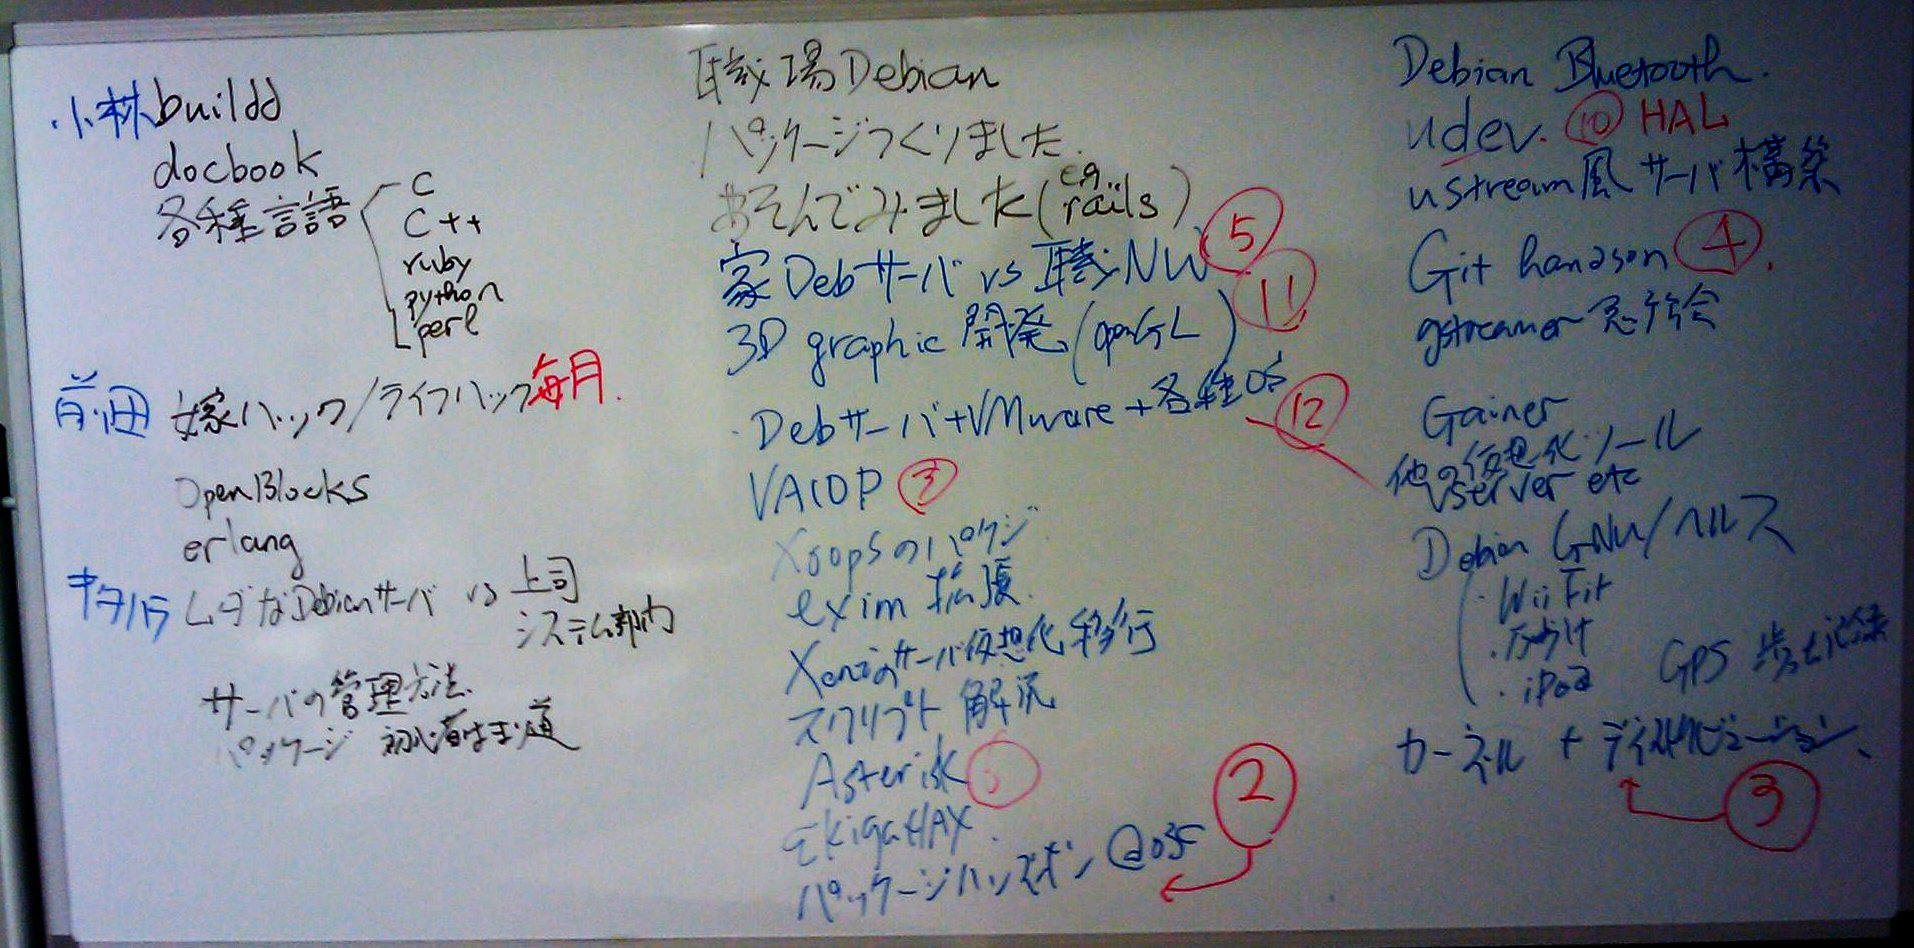
\includegraphics[width=1\hsize]{image200901/brainstorming.jpg}

\end{frame}

\begin{frame}{2009年計画}

{\scriptsize
 \begin{enumerate}
  \item 新年の企画 (アンサンブル荻窪開催)
  \item OSC Tokyo
  \item VAIO P インストール記録、
	カーネル読書会 ディストリビューション大集合(小林さん)(東京大学?)
  \item Git Handson (岩松)(あんさんぶる荻窪?)
  \item 家Debianサーバ vs 職場のネットワーク(千代田区都立図書館?\footnote{\url{http://www.library.chiyoda.tokyo.jp/}})
  \item Asterisk (東京大学?)
  \item スペインにて開催
  \item Debconf報告会
  \item OSC Fall?
  \item udev + HAL
  \item 3D graphics 開発
  \item Debian サーバ+VMware + 各種OS、
	他の仮想化ツール(vserver etc.)、
	忘年会
 \end{enumerate}
}
\end{frame}

\begin{frame}{2009年からのフロー(案)}

\begin{itemize}
 \item 前回の勉強会で発表内容を打ち合わせ (2/21)
 \item 二週間後にドラフト作成 (3/7)
 \item 三週間後に資料のテクニカルレビュー・メーリングリストで議論 (3/8-3/14)
 \item 印刷発注準備 (3/15-3/19)
 \item 四週間後に発表 (3/21)
\end{itemize}

\end{frame}

\emtext{冬休みの宿題}

\begin{frame}{}

楽しかった冬休みももう終わりました。
どんなDebianハックをしたのか、
冬休みの宿題、ということで発表してもらいます。

\begin{itemize}
 \item 上川純一
 \item 前田耕平
 \item 小室文
 \item id774
 \item 山本浩之
 \item 岩松信洋
\end{itemize}

\end{frame}

\emtext{上川純一}

\begin{frame}{Debian 勉強会資料 Git ワークフロー}

2008年10月の資料から Git format-patch で事前課題提出を依頼

うまくコンフリクトを解消できないなどの事例多数

どうする?

\end{frame}

\begin{frame}[containsverbatim]{ブランチで作業する}

毎月 git format-patch のためのブランチを作成する

\begin{commandline}
$ git pull
$ git checkout -b newbranch
\end{commandline}

master にはマージされた後の内容が反映される
\end{frame}

\begin{frame}{マージング}

\begin{minipage}{0.5\hsize}
 \includegraphics[height=0.8\vsize]{image200901/gitbranch.eps}
\end{minipage}
\begin{minipage}{0.4\hsize}
 \begin{itemize}
  \item マージ専用の捨てブランチをつくる
  \item master は alioth のツリーの内容にしておく
 \end{itemize}
\end{minipage}


\end{frame}

\emtext{前田耕平}

\begin{frame}{}

 \begin{center}

 黒 MacBook の Lenny/Sid 64bit 化 でのハマりポイント

 まえだこうへい mkouhei@debian.or.jp\\IRC nick: mkouhei
\end{center}


\end{frame}

\section{}
\begin{frame}
 \frametitle{Agenda}
  \begin{enumerate}
  \item 用意したインストールイメージ
  \item 簡単なインストール手順
  \item 起動させると…。
  \item 回避方法
  \item もっと簡単な回避方法。
 \end{enumerate}
\end{frame}

\section{事前準備}

\begin{frame}
 \frametitle{用意したインストールイメージ}
  \begin{itemize}
  \item Lenny のスナップショットイメージ

Debian GNU/Linux testing ''Lenny'' - Official Snapshot amd64
	 NETINST Binary-1 20090104-09:09

 \end{itemize}
\end{frame}

\section{手順}
\begin{frame}
 \frametitle{簡単なインストール手順}
 \begin{enumerate}
  \item expert install での起動。
  \item 日本語ロケール、米国キーボードを指定。
  \item パーティションの指定し直し。
  \item 基本パッケージのインストール。
  \item シェルモードへ移行。
  \item gptsync, refit パッケージのインストール、 gptsync の実行。
  \item apt-line の変更、apt-get \{update,upgrade,dist-upgrade\}の実行。
  \item 再起動。
 \end{enumerate}
\end{frame}

\section{Kernel Panic}

\begin{frame}[containsverbatim]
\frametitle{起動させると…。}
Kernel Panic となってしまいます。
\begin{commandline}
RAMDISK: Couldn't find valid RAM disk image staring at 0.
List of all partitions:
No filesystem could mount root, tried:
Kernel panic - not syncing: VFS: Unable to mount root fs on
 unknown-block(8,4)
\end{commandline}

\end{frame}

\begin{frame}[containsverbatim]
\frametitle{回避方法}
\begin{itemize}
\item レスキューモードで起動。
\item シェルモードになり、 /target へ chroot 。
\item カーネルソースを展開。
\item /boot 以下の該当の kernel config をカーネルソースツリーにコピー。
\item kernelをビルドし、インストール。
\begin{commandline}
REVISION=$(date +%Y%m%d.%H%M)
make-kpkg --initrd --revision $REVISION kernel_image
dpkg -i ../kernel-image-2.6.26_20090105.2330_amd64.deb
\end{commandline}

\item /ramdisk ディレクトリを作り、 initrd を展開。
\begin{commandline}
mkdir /ramdisk
cd /ramdisk
zcat /boot/initrd-2.6.26 | cpio -i
\end{commandline}
\end{itemize}
\end{frame}

\begin{frame}[containsverbatim]
\frametitle{回避方法(cont.)}
\begin{itemize}
\item 先ほどインストールした kernel をアンインストール。
\begin{commandline}
dpkg --purge kernel-image-2.6.26
\end{commandline}
\item .config の ''INITRAMFS\_SOURCE'' を書き換え、--initrd オプションな
      しで kernel をリビルド。
\begin{commandline}
sed -i 's:INITRAMFS_SOURCE="":INITRAMFS_SOURCE="/ramdisk":' .config
make-kpkg --revision $REVISION kernel\_image
\end{commandline}
\item できた kernel パッケージをインストール。
\item lilo.conf の ''initrd=/initrd.img'' をコメントアウトし、liloを書き
      込み。
\end{itemize}

\end{frame}

\begin{frame}[containsverbatim]
\frametitle{もっと簡単な回避方法。}
\textbf{ lilo をやめて、grub2 にしてしまいましょう。}

\begin{commandline}
# apt-get install grub-pc
# update-grub
# grub-install /dev/sda3
\end{commandline}

これで、initrdを作ってもちゃんとブートできます。


\end{frame}


\emtext{小室文}

\begin{frame}{}

\begin{center}

 {NamazuみたいにGoogle AJAX Search API}

 小室文
\end{center}

\end{frame}


\begin{frame}{自己紹介}
 小室 文

 aya@popowa.com
\end{frame}

\begin{frame}{目的}

 自分のウェブサイトの検索用にわざわざNamazuを導入しなくても
 \begin{enumerate}
 \item サイト内検索の機能を
 \item 簡単に
 \item デザインもカスタマイズ
 \end{enumerate}
 したかった。
\end{frame}

\begin{frame}{Google AJAX Search API}

 選択肢
 \begin{enumerate}
 \item JavaScriptあり
 \begin{enumerate}
 \item 自分でJavaScriptを組む
 \item ウィザードを使う
 \end{enumerate}
 \item JavaScriptなし
 \end{enumerate}
 基本的にHTMLファイル(もしくはPHPなど)をウェブサーバに置けば動きます。

\end{frame}

\begin{frame}{JavaScriptあり、なし両方}

 Google AJAX Search APIのKEYを事前に取得しておきます。
 \begin{enumerate}
 \item Google アカウント
 \item 使いたいFQDN
 \item 利用承諾に同意
 \end{enumerate}
 でKeyが発効されます。
\end{frame}

\begin{frame}{JavaScriptあり}

 \begin{enumerate}
 \item HTMLファイルの中で Google AJAX Search API JavaScript ライブラリをロード
 \item 検索をするオブジェクトを作成
 \item 検索準備(サーチャーメソッド追加、表示オプション、サイト制限設定など)
 \item 検索する
 \end{enumerate}
\end{frame}

\begin{frame}{JavaScriptなし}

 \begin{enumerate}
 \item \url{http://ajax.googleapis.com/ajax/services/search/web}
 に引数を渡してリクエスト
 \item JSON形式でレスポンスが得られる
 \item 見やすいように処理
 \end{enumerate}
\end{frame}


\begin{frame}{パラメーター}

 \begin{tabular}{|l|l|}
 \hline
 パラメータ & 項目 \\
 \hline
   q? & 検索したいキーワード、検索式\\
 \hline
   v=1.0 & プロトコル番号の指定 \\
 \hline
   key? & Google AJAX Search APIのKey\\
 \hline
   start? & 検索結果の開始インデックス\\
 \hline
   cx? & カスタム検索エンジンのID\\
 \hline
   lr? & 特定の言語のドキュメントを検索対象とする \\
 \hline
 \end{tabular}

\end{frame}

\begin{frame}[containsverbatim]{JavaScriptなし:レスポンス形式}

\begin{commandline}
{"responseData": {
"results": [
 {
  "GsearchResultClass": "GwebSearch",
  "unescapedUrl": "http://en.wikipedia.org/wiki/Paris_Hilton",
  "url": "http://en.wikipedia.org/wiki/Paris_Hilton",
  "visibleUrl": "en.wikipedia.org",
  "cacheUrl": "http://www.google.com/search?q\u003dcache:TwrPfhd22hYJ:en.wikipedia.org",
  "title": "\u003cb\u003eParis Hilton\u003c/b\u003e - Wikipedia, the free encyclopedia",
  "titleNoFormatting": "Paris Hilton - Wikipedia, the free encyclopedia",
  "content": "\[1\] In 2006, she released her debut album..."
 },
 ...
],
"cursor": {
 "pages": [
  { "start": "0", "label": 1 },
  { "start": "4", "label": 2 },
  { "start": "8", "label": 3 },
  { "start": "12","label": 4 }
 ],
 "estimatedResultCount": "59600000",
 "currentPageIndex": 0,
 "moreResultsUrl": "http://www.google.com/search?oe\u003dutf8\u0026ie\u003dutf8..."
}
}
, "responseDetails": null, "responseStatus": 200}
\end{commandline}

\end{frame}

\begin{frame}[containsverbatim]{現状の問題点}

 Google AJAX Search APIのかえしてくる「検索結果」の総数には問題があります。

 JavaScriptあり:
 setSiteRestrictionでドメインを指定して検索をしようとした
 場合、検索結果の総数が検索するたびに変わります。

 JavaScriptなし:
 \verb!?q=DMC\%20site:http://www.debian.or.jp/!とするとドメイン検索は出来
 るが、
 \verb!start?!で引数を渡すたびに同じように結果総数が変わります。

\end{frame}

\begin{frame}{まとめ}

当初の目的は達成出来ませんでした。

\begin{enumerate}
\item estimatedResultCountはestimateらしいです。
\item Yahoo Web検索でも発生します。
\item Yahoo!は検索リクエストがある度に検索結果を積算している、と免責してます。
\end{enumerate}

\end{frame}

\emtext{id774}
\emtext{山本 浩之}

\section{岩松信洋}
\emtext{岩松信洋}

\begin{frame}{}

\begin{center}
  Linuxカーネルコンフィグ変換ツール\\を作ってみた

\vspace{1em}

 岩松 信洋 iwamatsu@debian.or.jp\\IRC nick: iwamatsu

\end{center}

\end{frame}

\emtext{冬休み}
\section{赤ちゃんが生まれました}
\begin{frame}[containsverbatim]{赤ちゃんが生まれました}
赤ちゃんが生まれたので、世話をしていました。
 \begin{center}
 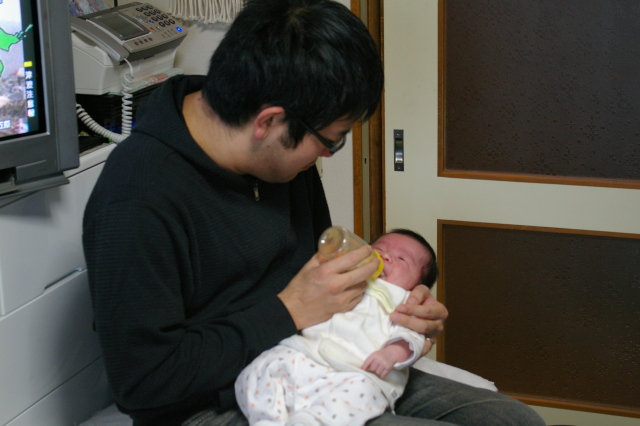
\includegraphics[scale=0.5]{image200901/baby.jpg}
 \label{fig:baby}
 \end{center}
\end{frame}

\emtext{今回作ったもの}
\section{今回作ったもの}
\begin{frame}[containsverbatim]{今回作ったもの}
\begin{center}\bfseries
システム情報を元に\\
システムに必要なカーネルモジュールを\\
組み込み指定に変換した\\
カーネルコンフィグファイルを出力する\\
スクリプト
\end{center}
\end{frame}
\begin{frame}[containsverbatim]{今回作ったもの}
\begin{center}
たいしてものではないです
\end{center}
\end{frame}


\begin{frame}{なぜこれを作ろうと思ったのか}
\begin{enumerate}
\item ひさびさにあまり使ってないマシンのカーネルコンフィグレーションをした。
\item コンフィグレーションが多すぎる。
\item 特にPCだと何を指定していいものやら。
\item 自動化できるんじゃね?
\item 自分は正規表現が苦手。正規表現の勉強のため。
\item Perlを学習する必要があった。
\item これらができて、アウトプットのできるものを作りますか。
\item 帰省の新幹線内で。
\end{enumerate}
\end{frame}

\begin{frame}{これができると}
\begin{enumerate}
\item カーネルコンフィグに悩まされずにすむ
\item 取り合えず動くカーネルはできる(はず)
\item 一般ユーザからvanilaカーネルアクセスへの敷居が下がる(かも)
\end{enumerate}
\end{frame}

\section{なぜ彼らはカーネルをリコンパイルするのか?}
\begin{frame}[containsverbatim]{}
\begin{center}
\large\bfseries
そういや、カーネルコンパイル!コンパイル!ってうるさい人たちいるよね?
\end{center}
\end{frame}

\begin{frame}[containsverbatim]
\begin{center}
\large\bfseries
なぜ彼らはカーネルをリコンパイルするのか?
\end{center}
\end{frame}

\begin{frame}{カーネルをリコンパイルする理由}
\begin{itemize}
\item カーネルハックのため。
\item カーネルBTSの深追い。
\item 最新のカーネルは新しいドライバや機能が使えるから。
\item ドライバを組み込みにして、起動の高速化。
\item ドキドキ感を味わうことができる。
\item 無駄にCPUを使いたい。(反エコ)
\end{itemize}
\end{frame}

\begin{frame}{カーネルをリコンパイルすることによるデメリット}
\begin{itemize}
\item 失敗したら動かなくなるかもしれない。
\item コンパイルにCPUリソースを食いすぎる(CPUが遅いため)。
\end{itemize}
\end{frame}

\begin{frame}{なぜ彼らはカーネルをリコンパイルするのか?}
\begin{center}
\large\bfseries
ここにいるひとたちには\\
後者なんて気にしないと思いますが。
\end{center}
\end{frame}

\emtext{内容}

\begin{frame}[containsverbatim]{必要なデータ}

\begin{itemize}
\item 使うカーネル\\
      Debianで提供しているカーネル(lenny では 2.6.26)
\item 入力するデータ
\begin{enumerate}
  \item カーネルソースコード
  \item 動いているカーネルのコンフィグファイル\\
	\url{/boot/config-2.6.26-1-xxx}
  \item システム情報
\end{enumerate}
\item 出力されるデータ\\
      システム情報を元にシステムに必要なカーネルモジュールが組み込み
      状態になっているカーネルコンフィグファイル
\end{itemize}
\end{frame}


\subsection{システム情報の取得方法}
\begin{frame}[containsverbatim]{システム情報の取得方法}
どのようにして、システム情報を取得するか。

\begin{table}[h]
 \begin{center}
 {
   \begin{tabular}{l|l} \hline
     コマンド & 内容  \\ \hline \hline
     dmidecode & BIOS からシステム情報を出力する \\
     lspci & PCI の情報を出力する \\
     lsusb & USB の情報を出力する \\
     dmesg & カーネルデバッグメッセージを出力する \\
     lsmod & ロードしてるモジュールを出力する \\
   \end{tabular}
 }
 \caption{起動しているカーネルから得られる情報}
 \label{kernel-output}
 \end{center}
\end{table}

\end{frame}

\subsection{システム情報の取得方法}
\begin{frame}[containsverbatim]{システム情報の取得方法}

今回利用したもの

\begin{table}[h]
 \begin{center}
 {
   \begin{tabular}{l|l} \hline
     コマンド & 内容  \\ \hline \hline
     lsmod & ロードしてるモジュールを出力する \\
   \end{tabular}
 }
 \caption{起動しているカーネルから得られる情報}
 \label{kernel-output}
 \end{center}
\end{table}


{\bf ロードしているモジュール=現在の Linux システムに必要なもの}
なので、わかりやすい。
\end{frame}

\emtext{簡単な流れ}

\begin{frame}{簡単な流れ}
1. データとして、
\begin{enumerate}
\item カーネルソースコードへのパス
\item 動作しているカーネルコンフィグファイル
\item lsmod の出力結果
\end{enumerate}
を指定する。

\end{frame}

\begin{frame}[containsverbatim]{簡単な流れ}
2. lsmod からロードしているドライバモジュール一覧を取得する

lsmod を実行すると、以下のような内容が出力される。
\begin{commandline0}
$ lsmod
Module                  Size  Used by
i915                   25280  2
drm                    65256  3 i915
ipv6                  235300  10
rfcomm                 28272  2
l2cap                  17248  9 rfcomm
........
\end{commandline0}
\end{frame}

\begin{frame}[containsverbatim]{簡単な流れ}

{\bf 3. ドライバモジュール名 と modinfo コマンドから ドライバモジュールのパスを取得する。}
\\

modinfo コマンドを使うと、指定したドライバモジュール名の情報を取得するこ
       とができます。-n オプションを使うと、ドライバオブジェクトファイル
       のパスが出力される。

\begin{commandline0}
$ modinfo -n i915
/lib/modules/2.6.26-1-amd64/kernel/drivers/char/drm/i915.ko
\end{commandline0}
\end{frame}

\begin{frame}[containsverbatim]{簡単な流れ}
\begin{commandline0}
$ modinfo -n i915
/lib/modules/2.6.26-1-amd64/kernel/drivers/char/drm/i915.ko
\end{commandline0}
 上の結果を例にすると、{\bf /lib/modules/2.6.26-1-amd64/kernel/} 以下と カーネルソース
 コードのパス構造は同じなため、ドライバモジュール名{\bf i915}の Makefile
 のあるパスは {\bf drivers/char/drm/Makefile} になる。

また、ドライバオブジェクトファイルは {\bf i915.ko} であることが分かる。
\end{frame}


\begin{frame}[containsverbatim]{簡単な流れ}

{\bf 4. 先で取得したMakefile へのパスとドライバオブジェクトファイル名より、
      対象になるドライバコンフィグ名を取得する。}

      ドライバオブジェクトファイル(i915.ko)とドライバモジュール名(i915)
      は必ずしも一致するとは限らないので、ドライバモジュール名を使って、
      ドライバコンフィグ名を検索する。(例えば snd\_hda\_intel)

\begin{commandline0}
.....
obj-$(CONFIG_DRM_I830)  += i830.o
obj-$(CONFIG_DRM_I915)  += i915.o <- これ
obj-$(CONFIG_DRM_SIS)   += sis.o
.....
\end{commandline0}
\end{frame}

\begin{frame}[containsverbatim]{簡単な流れ}

{\bf 5. 取得したドライバコンフィグ名を保存する。}
\end{frame}

\begin{frame}[containsverbatim]{簡単な流れ}

{\bf 6. 動作しているカーネルコンフィグファイルのドライバコンフィグを書き換える。}

正規表現を使って書き換えると、以下のようになる。
{\bf m} はモジュールを意味し、{\bf y} は組み込みを意味する。

変更前
\begin{commandline0}
....
CONFIG_DRM_I830=m
CONFIG_DRM_I915=m
CONFIG_DRM_MGA=m
....
\end{commandline0}

変更後
\begin{commandline0}
....
CONFIG_DRM_I830=m
CONFIG_DRM_I915=y <- 書き換え
CONFIG_DRM_MGA=m
....
\end{commandline0}
\end{frame}

\begin{frame}[containsverbatim]{簡単な流れ}

{\bf 7. 変更したものをファイルに出力する。}

\end{frame}


\emtext{実際に使ってみる}

\begin{frame}[containsverbatim]{ 実際に使ってみる}
\begin{commandline0}
$ moge -h
moge - Script to Kernel Module Enabler from lsmod command output

Copyright (C) 2008,2009 Nobuhiro Iwamatsu <iwamatsu@nigauri.org>
Usage: moge [options]
	-c, --configfile <file>   Kernel config file name
	-k, --kernel              Kernel source path
	-o, --output <file>       outout file
	-l, --lsmod               lsmod command output file
	-h, --help                display this help screen and exit
	-v, --version             show the version and exit

By Nobuhiro Iwamatsu <iwmatsu@nigauri.org>
$ moge -o sage -c config-2.6.26-1-686 -l lsmod.list -k \
                         /usr/src/linux-2.6-2.6.26/
\end{commandline0}
\end{frame}


\emtext{作成されたコンフィグファイルを使ってカーネルをコンパイルする}

\begin{frame}[containsverbatim]{カーネルコンパイルをする}
作成されたコンフィグファイルを使ってカーネルをコンパイルしてみる。

\begin{commandline0}
$ sudo apt-get update
$ sudo apt-get install linux-source-2.6.26 kernel-package
$ cd /usr/src/linux-source-2.6.26
$ make oldconfig
$ fakeroot make-kpkg --revision=yourpc00 kernel_image kenrel_header
$ ls ../
linux-image-2.6.26_yourpc00_i386.deb
linux-headers-2.6.26_yourpc00_i386.deb
.......
\end{commandline0}
\end{frame}

\section{変更結果}
\begin{frame}[containsverbatim]{lsmodの結果}

eeePC で試してみて、どれぐらい変わったのか調べてみた。

変更前 61モジュール
\begin{commandline0}
$ lsmod
Module                  Size  Used by
i915                   25280  2
drm                    65256  3 i915
ipv6                  235300  10
rfcomm                 28272  2

......

ide_core               96168  1 ide_pci_generic
ehci_hcd               28428  0
uhci_hcd               18672  0
usbcore               118160  5 uvcvideo,usb_storage,ehci_hcd,
uhci_hcd
thermal                15228  0
processor              32576  2 thermal
fan                     4164  0
thermal_sys            10856  4 video,thermal,processor,fan
\end{commandline0}
\end{frame}

\begin{frame}[containsverbatim]{lsmodの結果}

 変更後 0モジュール
\begin{commandline0}
$ lsmod
Module                  Size  Used by
\end{commandline0}

\end{frame}

\begin{frame}{bootchart}

{\bf bootchartでどれぐらい起動が速くなったか、調べてみました。}

\end{frame}

\begin{frame}{bootchart 変更前}
\begin{figure}
 \begin{center}
 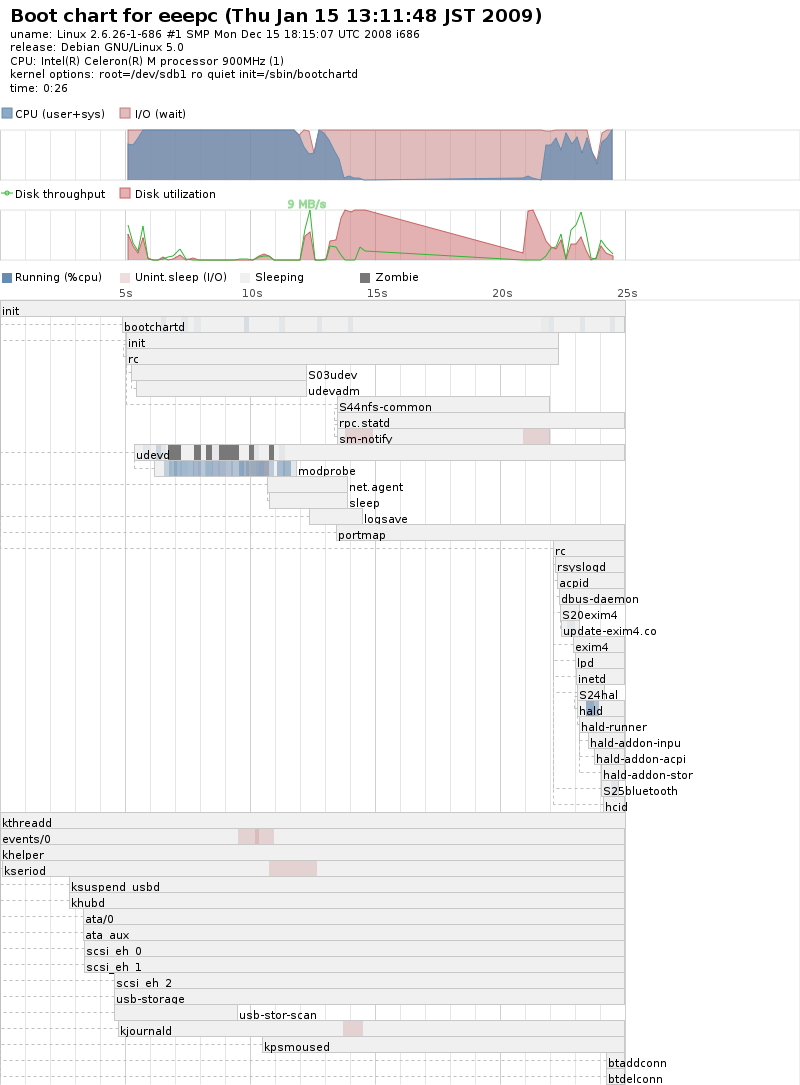
\includegraphics[scale=1.0]{image200901/bootchart-eeepc.png}
 \caption{変更前のbootchart}
 \label{fig:bootchart-eeepc}
 \end{center}
\end{figure}

\end{frame}

\begin{frame}{bootchart 変更後}
\begin{figure}
 \begin{center}
 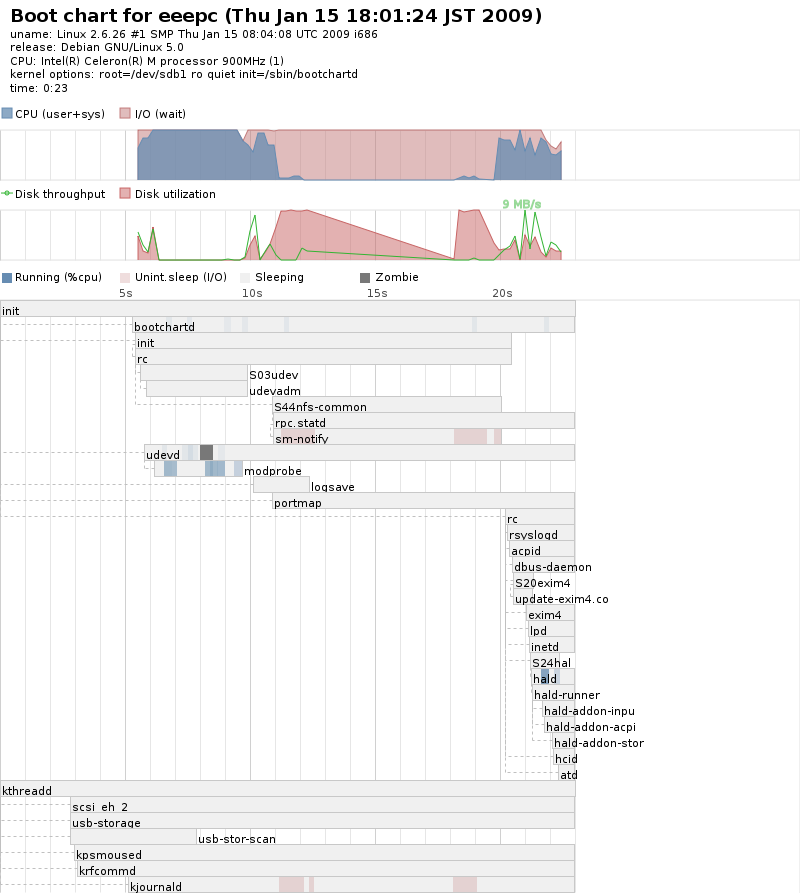
\includegraphics[scale=1.0]{image200901/bootchart-eeepc-new.png}
 \caption{変更後のbootchart}
 \label{fig:bootchart-eeepc-new}
 \end{center}
\end{figure}

\end{frame}

\begin{frame}{モジュールロード部分}
\begin{figure}
 \begin{center}
 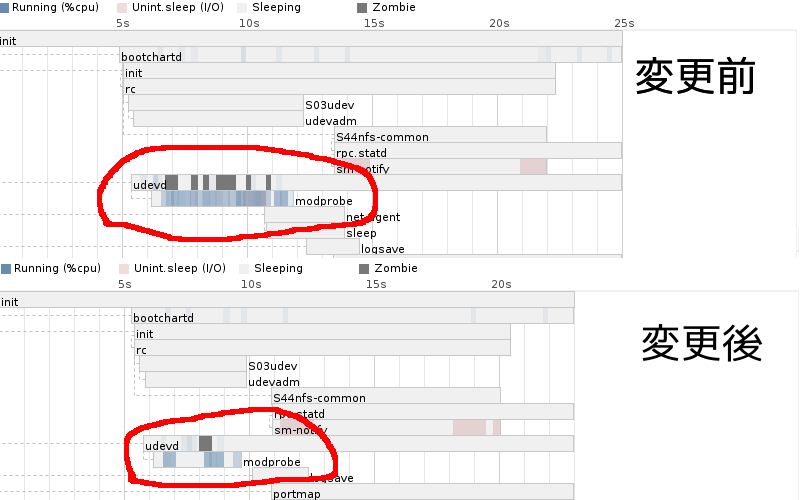
\includegraphics[scale=0.6]{image200901/bootchart-eeepc-merge.png}
 \caption{モジュールロード部分}
 \label{fig:bootchart-eeepc-merge}
 \end{center}
\end{figure}

\end{frame}


\section{今後の予定}
\begin{frame}{今後の予定}
\begin{enumerate}
 \item make-kpkg に入れる?
 \item パッケージ化?
 \item カーネルコンパイルWebサービスの提供?
 \item ドライバオブジェクトファイルとドライバモジュール名が一致しないやつを直す。
\end{enumerate}
\end{frame}

\emtext{次回の勉強会}
\begin{frame}{次回の勉強会}
次回 2008年2月 は OSC Tokyo です。

2008年3月21日は東京大学で開催予定です。

\end{frame}

\begin{frame}{宴会場所}
\begin{itemize}
 \item 宴会場所\\
       本日の宴会は「卯」です。\\
       参加者はフロアに集合し、全員で移動しましょう。
 \item 片付け\\
       部屋を片付けるのにご協力ください。
\end{itemize}
\end{frame}

\end{document}

;;; Local Variables: ***
;;; outline-regexp: "\\([ 	]*\\\\\\(documentstyle\\|documentclass\\|emtext\\|section\\|begin{frame}\\)\\*?[ 	]*[[{]\\|[]+\\)" ***
;;; End: ***
